\apendice{Experimentos sobre el algoritmo de división de texto}

En la sección de ``Codificación del texto'' del capítulo de ``Conceptos Teóricos'' de la Memoria, se introduce el problema que presentan muchos de los modelos de generación del lenguaje, entre ellos el modelo T5, el cual utilizamos. 

Dicho problema deriva del hecho de que estos modelos admiten un número de \emph{tókenes} de entrada máximo, 512 dn el caso del modelo T5.

Por tanto, desarrollamos un algoritmo que divide el texto en fragmentos, sin que ninguna frase quede partida, y siendo las diferencias entre el número de \emph{tókenes} en cada una de las divisiones tan pequeñas como sea posible.

Para ello, primero dividimos primero el texto de manera voraz, de forma que se van añadiendo frases a una subdivisión siempre que estas quepan sin ser fragmentadas. 

Esto puede resultar en que la última subdivisión contenga un número de frases muy inferior a la del resto de subdivisiones. Para solucionar este problema, se realiza un <<balanceo>> de las subdivisiones, moviendo frases de unas a otras, pero conservando su orden.

La \autoref{fig:balanceo} muestra el proceso de manera visual a través de un ejemplo:

\newpage

\begin{figure}[h!]
	\centering
	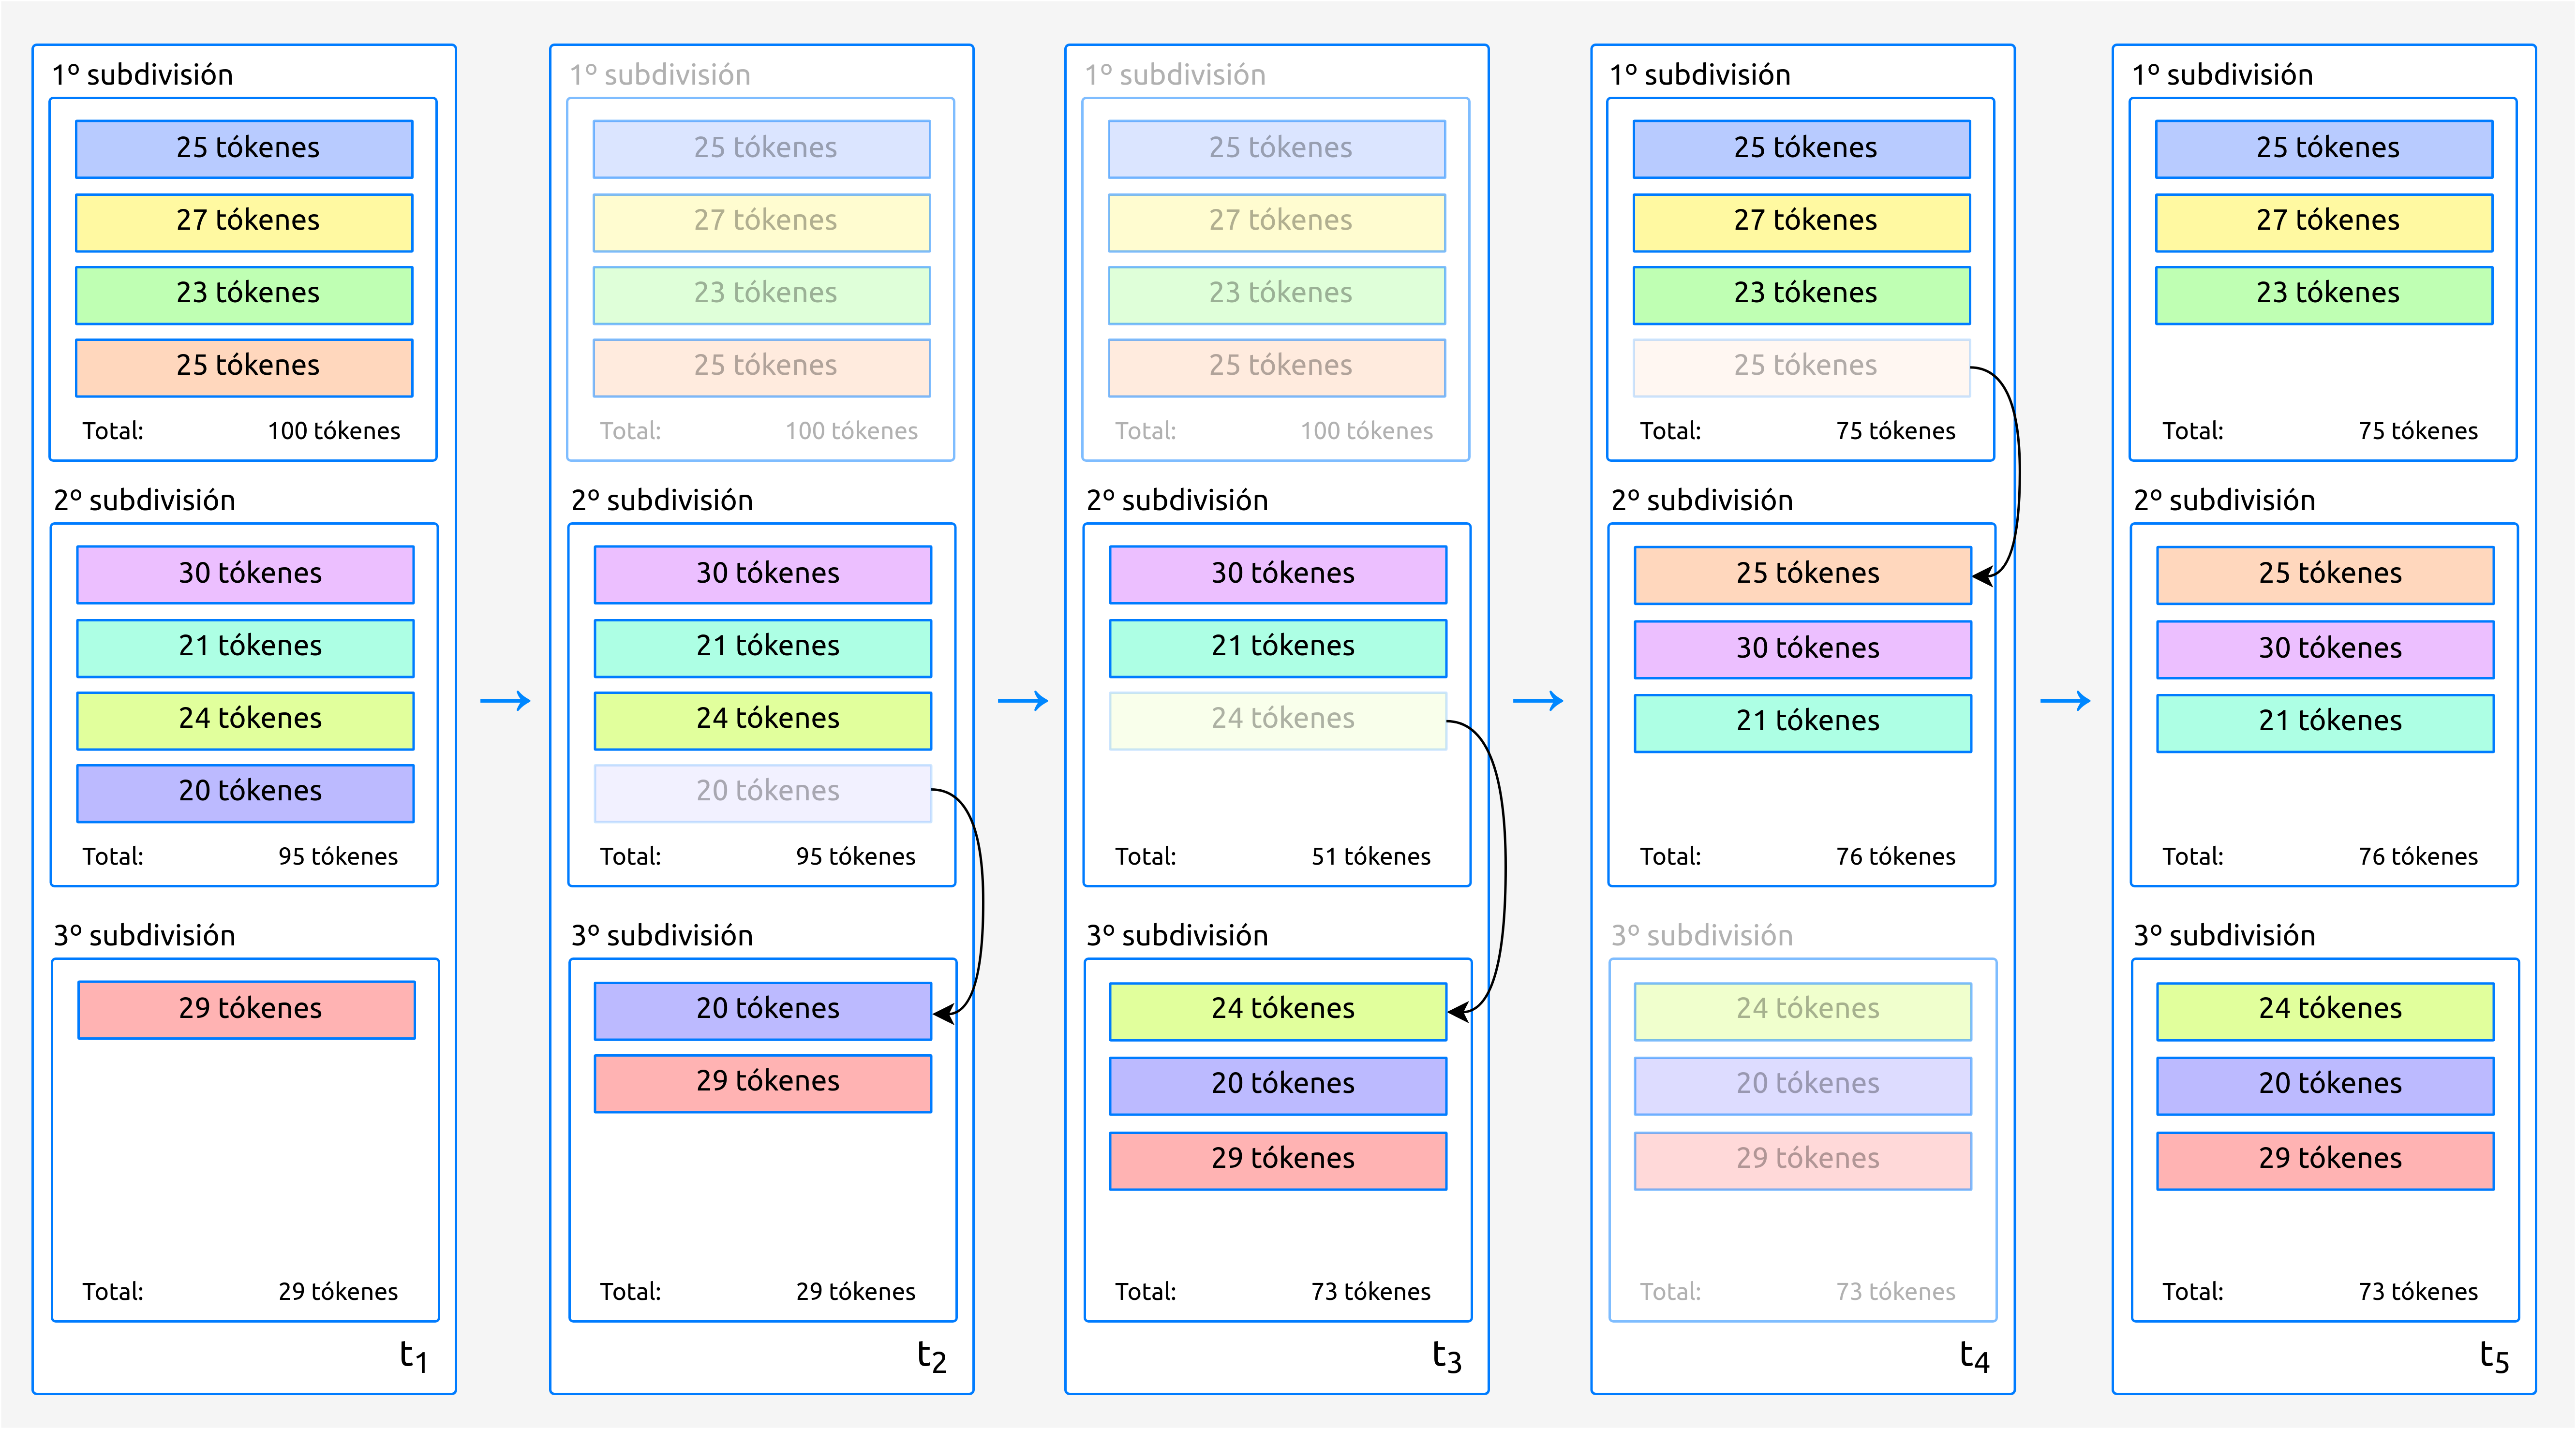
\includegraphics[width=\textwidth]{algoritmo-balanceo}
	\vspace{-0.5cm}
	\caption{Proceso de balanceo de las subdivisones generadas de forma voraz. Ejemplo con una longitud máxima de 100 \emph{tókenes}.}
	\label{fig:balanceo}
\end{figure}

En las tablas recogidas en las siguientes páginas, se muestra el número de \emph{tókenes} por subdivisión resultante de aplicar la división voraz, y el número de \emph{tókenes} por subdivisión una vez realizado el balanceo. Para los textos de los experimentos, se emplearon hilos de Twitter, teniendo el más corto 191 palabras, y artículos extraídos de Internet, el más largo de los cuales contiene 46.911 palabras.

Las diferencias entre el número de \emph{tókenes} antes y después de realizar la división  son claras, lo que indica el correcto funcionamiento del algoritmo propuesto. Además, el incremento de tiempo que introduce el balanceo es, por lo general, mínimo\footnote{\, Posteriormente a la realización de este experimento, se optimizó notablemente el rendimiento global del algoritmo para el modelo T5. Para más información, se puede consultar la siguiente \emph{Issue} en el repositorio del proyecto en GitHub: \href{https://github.com/dmlls/jizt/issues/97}{https://github.com/dmlls/jizt/issues/97}.}.

\newpage

\begin{table}[h!]
	\centering
	\begin{tabular}{>{\centering}b{0.09\linewidth}>{\raggedright}b{0.18\linewidth}>{\raggedright}b{0.3\linewidth}>{\raggedright\arraybackslash}b{0.3\linewidth}}
		\toprule
		\multicolumn{4}{c}{\large\textbf{\begin{minipage}{1\linewidth}\centering Codificación con división de texto \\ \small{(hilos reales de Twitter)} \end{minipage}}} \\
		\smallskip
		\scriptsize{Palabras/ \emph{tókenes}} & & Voraz & Balanceado \\
		
		\midrule
		
		\multirow{3}{*}{\begin{minipage}{0.5in}\centering 191 \\ \scriptsize{280} \\ \tiny{(4 tweets)} \end{minipage}}	& \small{Tokens/subdiv.} & \small{[280]} & \small{[280]} \\
		& \small{\textbf{Desv. estándar}} & \small{\textbf{0,0}} & \small{\textbf{0,0}} \\
		& \small{Tiempo} & \small{5,23 ms} & \small{5,25 ms} \\
		
		\midrule
		
		\multirow{3}{*}{\begin{minipage}{0.5in}\centering 394\\ \scriptsize{534} \\ \tiny{(11 tweets)} \end{minipage}}	& \small{Tokens/subdiv.} & \small{[506, 28]} & \small{[273, 261]} \\
		& \small{\textbf{Desv. estándar}} & \small{\textbf{239,0}} & \small{\textbf{6,0}} \\
		& \small{Tiempo} & \small{8,15 ms} & \small{8,21 ms} \\
		
		\midrule
		
		\multirow{3}{*}{\begin{minipage}{0.5in}\centering 646\\ \scriptsize{906} \\ \tiny{(16 tweets)} \end{minipage}}	& \small{Tokens/subdiv.} & \small{[504, 402]} & \small{[448, 458]} \\
		& \small{\textbf{Desv. estándar}} & \small{\textbf{51,0}} & \small{\textbf{5,0}} \\
		& \small{Tiempo} & \small{13,4 ms} & \small{13,8 ms} \\
		
		\midrule
		
		\multirow{3}{*}{\begin{minipage}{0.5in}\centering 1.089 \\ \scriptsize{1.417} \\ \tiny{(23 tweets)} \end{minipage}}	& \small{Tokens/subdiv.} & \small{[488, 477, 452]} & \small{[478, 487, 452]} \\
		& \small{\textbf{Desv. estándar}} & \small{\textbf{15,06}} & \small{\textbf{14,84}} \\
		& \small{Tiempo} & \small{26,10 ms} & \small{25,70 ms} \\
		
		\midrule
		
		\multirow{3}{*}{\begin{minipage}{0.5in}\centering 1.536\\ \scriptsize{2.069} \\ \tiny{(32 tweets)} \end{minipage}}	& \small{Tokens/subdiv.} & \small{[509, 508, 507, 501, 44]} & \small{[437, 419, 409, 407, 397]} \\
		& \small{\textbf{Desv. estándar}} & \small{\textbf{184,92}} & \small{\textbf{13,54}} \\
		& \small{Tiempo} & \small{41 ms} & \small{41,2 ms} \\
		
		\midrule
		
		\multirow{3}{*}{\begin{minipage}{0.5in}\centering 1.871\\ \scriptsize{4.531} \\ \tiny{(43 tweets)} \end{minipage}}	& \small{Tokens/subdiv.} & \small{[409, 426, ... , 475, 414]} & \small{[409, 426, ... , 422, 467]} \\
		& \small{\textbf{Desv. estándar}} & \small{\textbf{39,70}} & \small{\textbf{32,11}} \\
		& \small{Tiempo} & \small{34,7 ms} & \small{35,4 ms} \\
		
		\midrule
		
		\multirow{3}{*}{\begin{minipage}{0.5in}\centering 2,060\\ \scriptsize{3,255} \\ \tiny{(51 tweets)} \end{minipage}}	& \small{Tokens/subdiv.} & \small{[501, 497, ... , 402, 509]} & \small{[501, 497, ... , 402, 509]} \\
		& \small{\textbf{Desv. estándar}} & \small{\textbf{54,40}} & \small{\textbf{37,65}} \\
		& \small{Tiempo} & \small{26,1 ms} & \small{26,7 ms} \\
		
		\midrule
		
		\multirow{3}{*}{\begin{minipage}{0.5in}\centering 3,753\\ \scriptsize{5,293} \\ \tiny{(103 tweets)} \end{minipage}}	& \small{Tokens/subdiv.} & \small{[504, 505, ... , 503, 386]} & \small{[504, 505, ... , 469, 437]} \\
		& \small{\textbf{Desv. estándar}} & \small{\textbf{36,75}} & \small{\textbf{19,72}} \\
		& \small{Tiempo} & \small{62,1 ms} & \small{62,9 ms} \\
		
		\bottomrule
	\end{tabular}
	\caption{Resultados en la codificación de hilos de Twitter reales. Desviación estándar calculada sobre el número de \emph{tókenes} por subdivisión.}
\end{table}

\newpage


\begin{table}[h]
	\vspace{0.5cm}
	\centering
	\begin{tabular}{>{\centering}b{0.09\linewidth}>{\raggedright}b{0.18\linewidth}>{\raggedright}b{0.3\linewidth}>{\raggedright\arraybackslash}b{0.3\linewidth}}
		\toprule
		\multicolumn{4}{c}{\large\textbf{\begin{minipage}{1\linewidth}\centering Codificación con división de texto \\ \small{(textos muy largos)} \end{minipage}}} \\
		\smallskip
		\scriptsize{Palabras/ \emph{tókenes}} & & Voraz & Balanceado \\
		
		\midrule
		
		\multirow{3}{*}{\begin{minipage}{0.5in}\centering 5.022 \\ \scriptsize{8.051} \end{minipage}}	& \small{Tokens/subdiv.} & \small{[498, 499, ... , 497, 77]} & \small{[498, 499, ... , 418, 396]} \\
		& \small{\textbf{Desv. estándar}} & \small{\textbf{99,88}} & \small{\textbf{39,21}} \\
		& \small{Tiempo} & \small{118 ms} & \small{120 ms} \\
		
		\midrule
		
		\multirow{3}{*}{\begin{minipage}{0.5in}\centering 10.058 \\ \scriptsize{15.761} \end{minipage}}	& \small{Tokens/subdiv.} & \small{[498, 499, ... , 496, 415]} & \small{[498, 499, ... , 461, 484]} \\
		& \small{\textbf{Desv. estándar}} & \small{\textbf{23,54}} & \small{\textbf{15,52}} \\
		& \small{Tiempo} & \small{250 ms} & \small{251 ms} \\
		
		\midrule
		
		\multirow{3}{*}{\begin{minipage}{0.5in}\centering 20.203\\ \scriptsize{30.989} \end{minipage}}	& \small{Tokens/subdiv.} & \small{[498, 499, ... , 481, 311]} & \small{[498, 499, ... , 425, 420]} \\
		& \small{\textbf{Desv. estándar}} & \small{\textbf{29,51}} & \small{\textbf{18,95}} \\
		& \small{Tiempo} & \small{470 ms} & \small{488 ms} \\
		
		\midrule
		
		\multirow{3}{*}{\begin{minipage}{0.5in}\centering 46.911\\ \scriptsize{69.772} \end{minipage}}	& \small{Tokens/subdiv.} & \small{[498, 499, ... , 505, 121]} & \small{[498, 499, ... , 392, 385]} \\
		& \small{\textbf{Desv. estándar}} & \small{\textbf{35,05}} & \small{\textbf{17,01}} \\
		& \small{Tiempo} & \small{1,08 s} & \small{1,11 s} \\
		\bottomrule
	\end{tabular}
	\caption{Resultados en la codificación de textos muy largos. Desviación estándar calculada sobre el número de \emph{tókenes} por subdivisión.}
\end{table}